%
% File: chap02.tex
% Author: Abhushan Sahu
% Description: Introduction chapter where the stuff goes on.
%
\let\textcircled=\pgftextcircled
\chapter{Research}
\label{chap:intro}

\initial{F}or a project to sustain, there has to be some hard work done on it, that describes it.\\
 That background work has been listed in here. \\
 Research comprises ``creative work undertaken on a systematic basis in order to increase the stock of knowledge, including knowledge of humans, culture and society, and the use of this stock of knowledge to devise new applications.''


%=======
\section{Introduction}
\label{sec:sec01}

Research in this dissertation is done on newtonian physics, that deals with gravity(mainly).
Here earth's gravity has been removed for true acceleration value, by the formula.
\begin{equation}
\begin{split}
gx=0; \\
gy=0; \\
gz=0; \\
alpha=0.9; \\
gx=alpha * gx + (1 - alpha) * x; \\
gy=alpha * gy + (1 - alpha) * y; \\
gz=alpha * gz + (1 - alpha) * z; \\
x=x-gx; \\
y=y-gy; \\
z=z-gz; 
\end{split}
\end{equation}

\section{Recorded Data}
\label{sec:sec02}
{
The data provided are the Accelerometer Values.\\
The interval per data is of 30milliseconds. \\
The data recorded is done by: \\  
Sensor vendor: Bosch Sensortec GmbH*. \\
Name: BMA150 accelerometer. Type: 1. Version : 1\\ 
Range 9.81 $m/s^2$ \\
For the sake of briefness, the graph has been stacked/clustered, as the sample space consists of 1901 record entries.\\
X-axis denotes time, Y-axis denotes acceleration. \\
\vfill
*Gesellschaft mit beschrankter Haftung- German for ``company with limited liability''
\clearpage




\begin{figure}[!htb]
{	\centering
	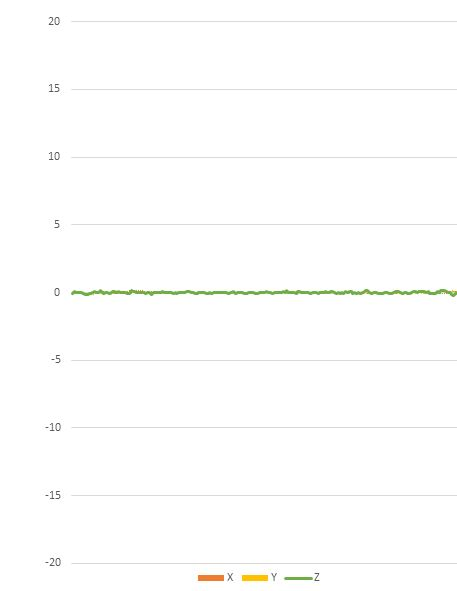
\includegraphics[height=0.35\textheight]{fig01/g_stable}
	\mycaption[Graph depicting rest.]{Graph depicting rest.}
	\label{fig:RHP01} \par\medskip
}



This state of rest is measured, when the phone is placed on a table, without any disturbance, (angle of placement doesn't matter.) \par\medskip
    
{
	\centering
	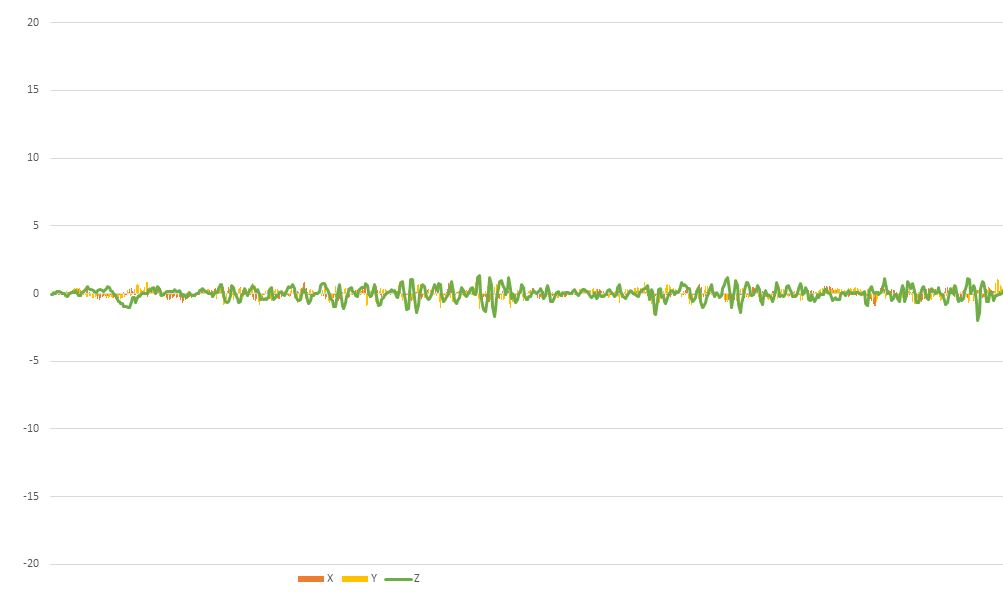
\includegraphics[height=0.35\textheight]{fig01/g_walk}
	\mycaption[Graph depicting a walk/normal walk.]{Graph depicting a walk/normal walk.}
	\label{fig:RHP02} \par\medskip
}


This state of motion, depicts a user to have a walk around the work-room/house with the device in either hands or in the pocket.\\
Though there would be an extended curve when placed inside pocket, but that is within the threshold value.
    
    
\end{figure}

\begin{figure}[h]


{
	\centering
	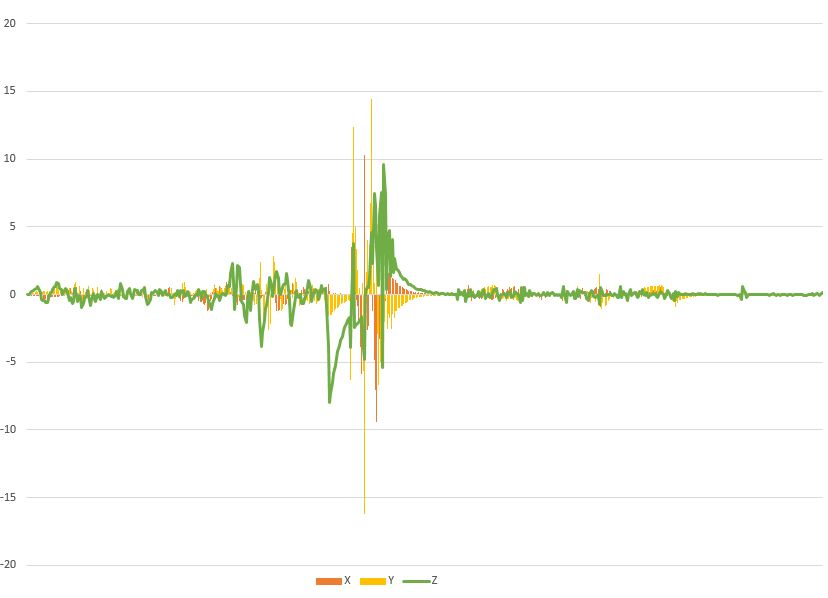
\includegraphics[height=0.35\textheight]{fig01/g_fall}
	\mycaption[Graph depicting a fall.]{Graph depicting a fall.}
	\label{fig:RHP03} \par
    }
    
  This state of fall, is measured in controlled condition, when the user has a phone with him, and the user undergoes a jerk in motion, the extremities which are shown here are the data of need. \\
There is a pattern in fall.   
\end{figure}
}


\section{Fall pattern}
\label{sec:sec03}
There is a certain pattern, a uniformity in fall.
If seen at the sample space, one can find that the acceleration suddenly increase.
But if seen more precisely, then it is clear, that there is a lot of things going on. \\
An accident or a mishap, or the counter for our action, generally comprises with a free-fall.
This free-fall, has a the following shape in the respective domain. Which is similar to the data been recorded.

\begin{figure}[h]


\centering
\begin{minipage}{3.3cm}
    \centering
    \subtop[]{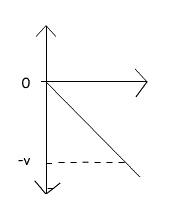
\includegraphics[height=0.28\textheight]{fig01/g_freefall_1}\label{sf:multiRH02a}}
\end{minipage}
\hspace{0.5cm}
\begin{minipage}{3.3cm}
    \centering
    \subtop[]{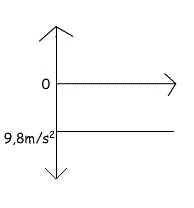
\includegraphics[height=0.27\textheight]{fig01/g_freefall_2}\label{sf:multiRH02b}}
\end{minipage}
\hspace{1.3cm}
\begin{minipage}{3.3cm}
    \centering
    \subtop[]{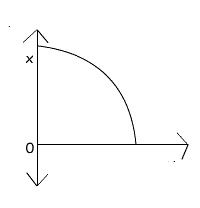
\includegraphics[height=0.27\textheight]{fig01/g_freefall_3}\label{sf:multiRH02c}}
\end{minipage}

\mycaption[Graph of Free-fall in terms of]{(a) Graph of Free-fall in terms of velocity/time. (b) Graph of Free-fall in terms of acceleration/time. (c) Graph of Free-fall in terms of position/time}
\label{fig:multiRH02}
\end{figure}
\clearpage

\section{Jerk Pattern}
\label{sec:sec04}
In addition to this free-fall, another counter that sets it off is the sudden deceleration. \\
We follow the pattern as: \\

\begin{figure}[h]
\centering
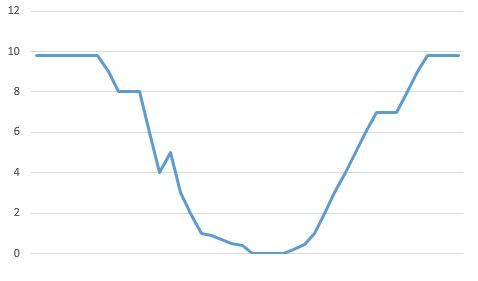
\includegraphics[height=0.35\textheight]{fig01/g_fall_G}
\mycaption[Graph for jerk in gravitational acceleration.]{Graph for jerk in gravitational acceleration.}
	\label{fig:RHP01}

\end{figure}

\begin{figure}[!b]

\centering
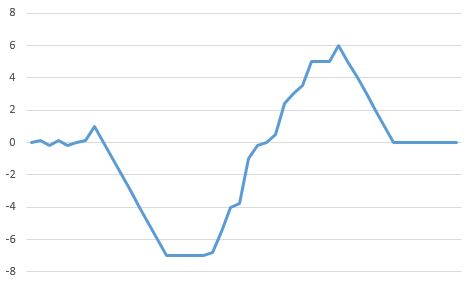
\includegraphics[height=0.35\textheight]{fig01/g_fall_A}
\mycaption[Graph for jerk in acceleration.]{Graph for jerk in acceleration.}
	\label{fig:RHP02}
This pattern sets the trigger for our response system. Though this finding acts as an upper-bound for the actual act. More processing and data-refinement needs to be done, and is under processing.
\end{figure}

